\chapter{Filesender}
Filesender est une application sécurisée d'envoi de transfert de fichiers volumineux proposée par Renater. 
Une fois le service sélectionné il s'effectue une redirection vers la sélection du guichet --~comprendre l'académie~-- d'authentification.
\begin{figure}
	\centering
	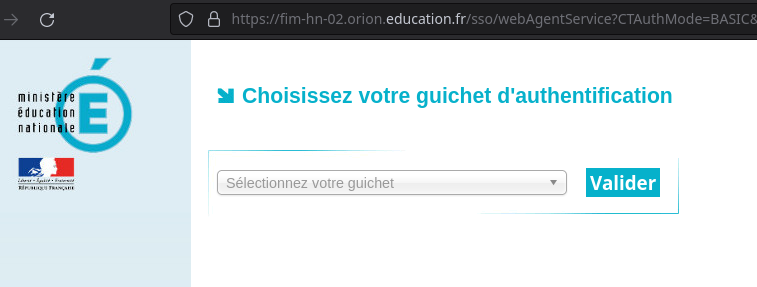
\includegraphics{./Captures/filesender.choix.guichet-academique.png}
%	\caption{}
\end{figure}
On se retrouve alors vers la fenêtre habituelle d'authentification des services académiques pour l'identifiant académique et le mot de passe correspondant.
\begin{figure}
	\centering
	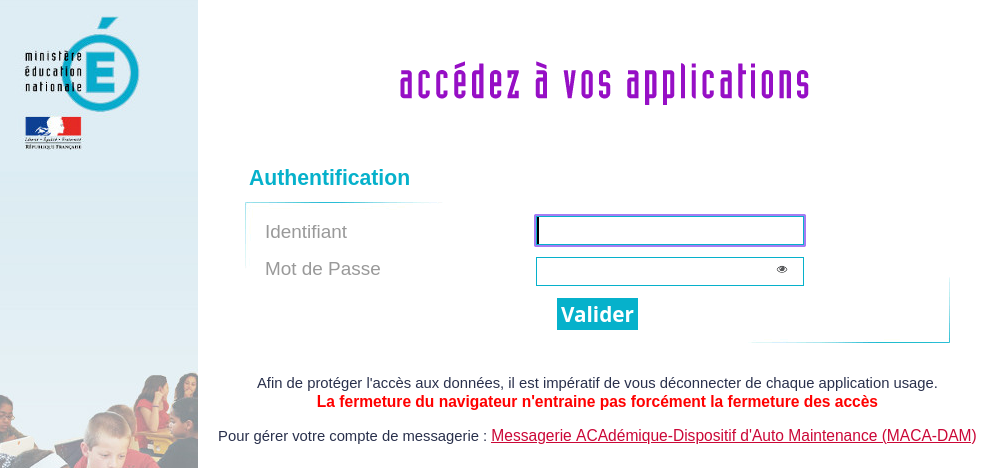
\includegraphics{./Captures/authentification.academique.png}
	\caption{}
\end{figure}
et bien entendu une fois l'authentification et l'identification faites, une redirection amènera l'utilisateur vers le portail
\begin{figure}
	\centering
	
\includegraphics{./Captures/authentification.academique.redirection.png}
%	\caption{}
\end{figure}
Pour finir, la page d'accueil du service s'affichera.
\begin{figure}
	\centering
	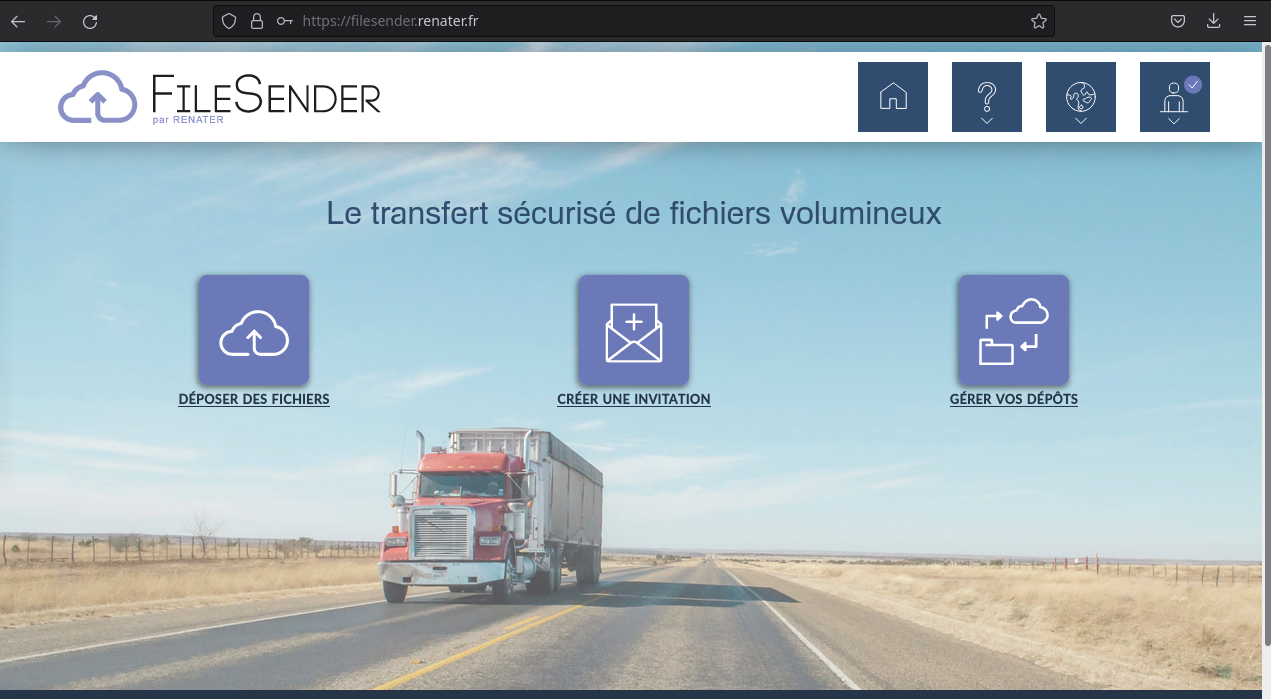
\includegraphics{./Captures/filesender.homepage.png}
	\caption{L'écran d'accueil de FileSender}
\end{figure}

L'interface de Filesender est très épurée, elle est constituée de 7 icônes à deux endroits différents, les 4 icônes à droite en haut correspondent aux accès suivants --~de gauche à droite~--
\begin{itemize}
	\item le retour à la page d'accueil,
	\item l'accès à l'aide en ligne, à savoir le guide de l'utilisateur, la foire aux questions et les conditions générales d'utilisation,
	\item le choix de la langue~: Français ou anglais,
	\item l'accès aux réglages du profil et la déconnexion du service.
\end{itemize}

Dans un premier temps, ce sont les trois icônes de la partie centrale, en les parcourant de gauche à droite, qui vont être étudiés individuellement. 
Par la suite, étant donné les options des icônes de la zone supérieure, je ne m'intéresserait qu'au profil de l'utilisateur, le reste étant finalement assez clair ou n'affichant pas de fenêtre particulière.

%filesender-deposer-fichier.tex
\section{Déposer des fichiers}

\begin{figure}
	\centering
	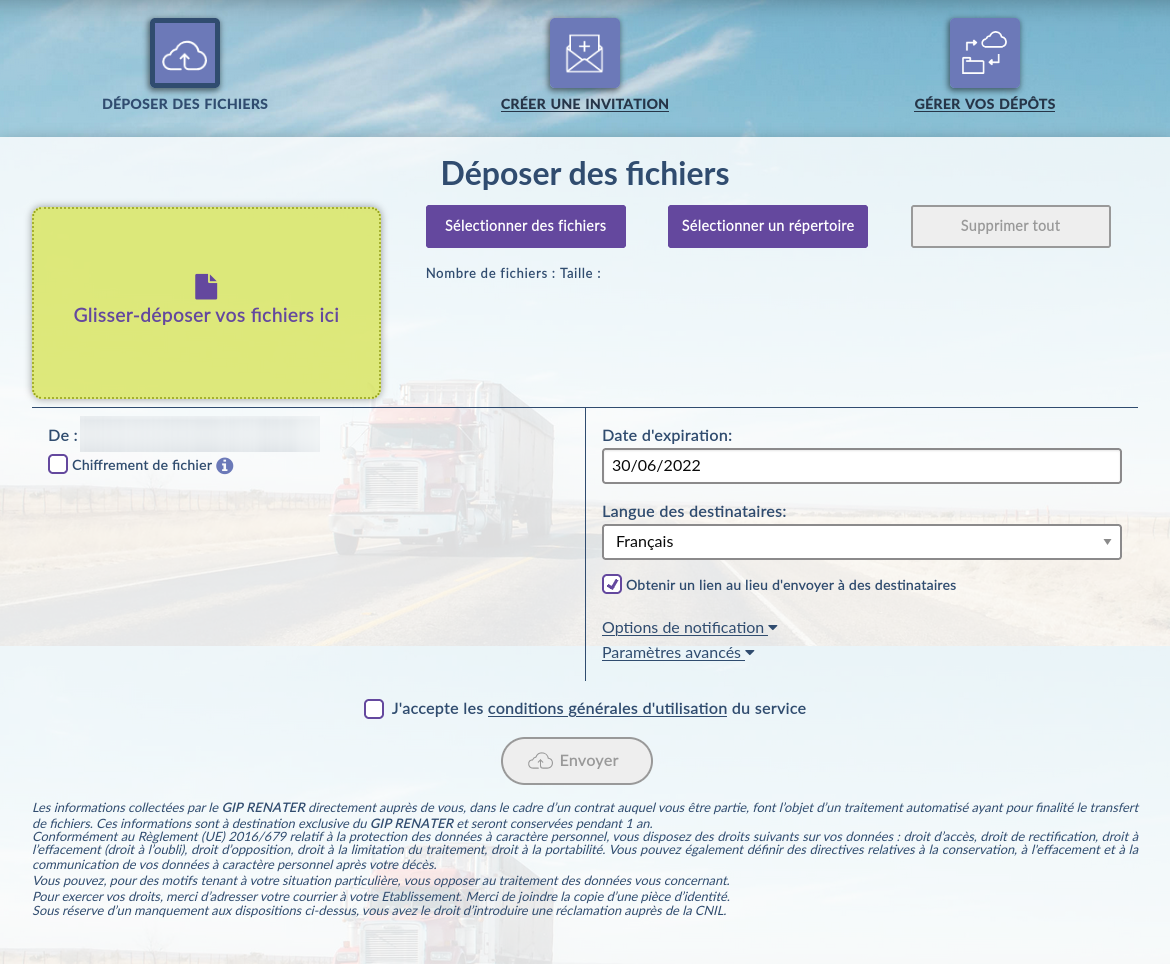
\includegraphics{./Captures/filesender.envoi.fichier.png}
%	\caption{}
\end{figure}


%\input{filesender-creer-invitation.tex}

%\input{filesender-gerer-depots.tex}

%\input{filesender-aides.tex}

%\input{filesender-langages.tex}

%\input{filesender-profil-utilisateur.tex}